\documentclass[11pt]{beamer}
\usepackage[utf8]{inputenc}
\usepackage{amsmath}
\usepackage{amsfonts}
\usepackage{amssymb}
\usepackage{graphicx}
\usepackage{listings}
\usepackage{tikz}
\usetikzlibrary{calc,shapes.geometric, arrows}
\usetheme{Hannover}
\begin{document}
	\author{Wang Xuanyu}
	\title{High Performance Parallel FDTD Computation by Using Vector Processor and CUDA}
	%\subtitle{}
	%\logo{}
	\institute{University of Electronic Science and Technology of China}
	\date{June 4 2016}
	\subject{Fundamental Science}
	%\setbeamercovered{transparent}
	%\setbeamertemplate{navigation symbols}{}
	\frame[plain]{\maketitle}
	\lstset{breaklines,tabsize=4,language=C,numbers=left,numberstyle=\tiny,backgroundcolor=\color{lightgray!40!white},extendedchars=false,keywordstyle=\color{blue!70}\bfseries,basicstyle=\tiny,commentstyle=\ttfamily\color{green!40!black}}
	
	
\section{Introduction}
	\begin{frame}
		\frametitle{FDTD}
		FDTD: Finite Difference Time Domain.
		\begin{figure}[hp]
			\centering
			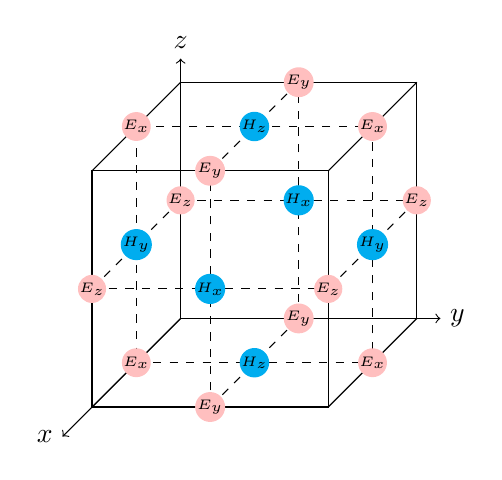
\begin{tikzpicture}
			\def \len {3}
			\def \hlen {1.5}
			\def \coe {-0.75}
			
			%back rectangle wigh dashline
			\draw(0,0) rectangle +(\len,\len);
			\draw [dashed] ($(0,0)+0.5*(0,\len)$) -- +(\len,0);
			\draw [dashed] ($(0,0)+0.5*(\len,0)$) -- +(0,\len);
			
			%front rectangle wigh dashline
			\draw($(0,0)+\coe*(\hlen,\hlen)$) rectangle +(\len,\len);
			\draw [dashed] ($(0,0)+(0,\hlen)+\coe*(\hlen,\hlen)$) -- +(\len,0);
			\draw [dashed] ($(0,0)+(\hlen,0)+\coe*(\hlen,\hlen)$) -- +(0,\len);
			
			%connect two rectangle
			\draw (0,0) -- ($(0,0)+\coe*(\hlen,\hlen)$);
			\draw ($(0,0)+(0,\len)$) -- ($(0,0)+(0,\len)+\coe*(\hlen,\hlen)$);
			\draw ($(0,0)+(\len,0)$) -- ($(0,0)+(\len,0)+\coe*(\hlen,\hlen)$);
			\draw ($(0,0)+(\len,\len)$) -- ($(0,0)+(\len,\len)+\coe*(\hlen,\hlen)$);
			
			%all dashline
			\draw [dashed] ($(0,0)+(0,\hlen)$) -- ($(0,0)+(0,\hlen)+\coe*(\hlen,\hlen)$);
			\draw [dashed] ($(0,0)+(\hlen,0)$) -- ($(0,0)+(\hlen,0)+\coe*(\hlen,\hlen)$);
			\draw [dashed] ($(0,0)+(\len,\hlen)$) -- ($(0,0)+(\len,\hlen)+\coe*(\hlen,\hlen)$);
			\draw [dashed] ($(0,0)+(\hlen,\len)$) -- ($(0,0)+(\hlen,\len)+\coe*(\hlen,\hlen)$);
			
			\draw [dashed] ($(0,0)+0.5*\coe*(\hlen,\hlen)$) -- ++(\len,0) -- ++(0,\len) -- ++(-\len,0) -- cycle;
			
			%axis
			\draw [->] (0,0) -- +(1.1*\len,0) node[right]{$y$};
			\draw [->] (0,0) -- +(0,1.1*\len) node[above]{$z$};
			\draw [->] (0,0) -- +($(0,0)-(\hlen,\hlen)$) node[below,left]{$x$};
			
			%nodes
			\begin{tiny}
			%Hx
			\node[shape=circle,fill=cyan,inner sep=0pt] at (\hlen,\hlen) {$H_x$};
			\node[shape=circle,fill=cyan,inner sep=0pt] at ($(\hlen,\hlen)+\coe*(\hlen,\hlen)$) {$H_x$};
			%Hz		
			\node[shape=circle,fill=cyan,inner sep=0pt] at ($(0,0)+(\hlen,0)+0.5*\coe*(\hlen,\hlen)$) {$H_z$};
			\node[shape=circle,fill=cyan,inner sep=0pt] at ($(0,0)+(\hlen,0)+0.5*\coe*(\hlen,\hlen)+(0,\len)$) {$H_z$};
			%Hy
			\node[shape=circle,fill=cyan,inner sep=0pt] at ($(0,0)+(0,\hlen)+0.5*\coe*(\hlen,\hlen)$) {$H_y$};
			\node[shape=circle,fill=cyan,inner sep=0pt] at ($(0,0)+(0,\hlen)+0.5*\coe*(\hlen,\hlen)+(\len,0)$) {$H_y$};
			%Ez
			\node[shape=circle,fill=pink,inner sep=0pt] at ($(0,\hlen)$) {$E_z$};
			\node[shape=circle,fill=pink,inner sep=0pt] at ($(0,\hlen)+\coe*(\hlen,\hlen)$) {$E_z$};
			\node[shape=circle,fill=pink,inner sep=0pt] at ($(0,\hlen)+(\len,0)$) {$E_z$};
			\node[shape=circle,fill=pink,inner sep=0pt] at ($(0,\hlen)+\coe*(\hlen,\hlen)+(\len,0)$) {$E_z$};
			%Ex
			\node[shape=circle,fill=pink,inner sep=0pt] at ($(0,\hlen)+0.5*\coe*(\hlen,\hlen)+(0,\hlen)$) {$E_x$};
			\node[shape=circle,fill=pink,inner sep=0pt] at ($(0,\hlen)+0.5*\coe*(\hlen,\hlen)+(\len,0)+(0,\hlen)$) {$E_x$};
			\node[shape=circle,fill=pink,inner sep=0pt] at ($(0,\hlen)+0.5*\coe*(\hlen,\hlen)+(0,-\hlen)$) {$E_x$};
			\node[shape=circle,fill=pink,inner sep=0pt] at ($(0,\hlen)+0.5*\coe*(\hlen,\hlen)+(\len,0)+(0,-\hlen)$) {$E_x$};
			%Ey
			\node[shape=circle,fill=pink,inner sep=0pt] at ($(\hlen,\hlen)+(0,\hlen)$) {$E_y$};
			\node[shape=circle,fill=pink,inner sep=0pt] at ($(\hlen,\hlen)+\coe*(\hlen,\hlen)+(0,\hlen)$) {$E_y$};
			\node[shape=circle,fill=pink,inner sep=0pt] at ($(\hlen,\hlen)+(0,-\hlen)$) {$E_y$};
			\node[shape=circle,fill=pink,inner sep=0pt] at ($(\hlen,\hlen)+\coe*(\hlen,\hlen)+(0,-\hlen)$) {$E_y$};
			\end{tiny}
			\end{tikzpicture}
			\caption{The spatial discrete structure of Yee cell}\label{yee cell}
		\end{figure}
	\end{frame}
	
	\begin{frame}{Vector Processor}
	\begin{figure}[hp]
		\centering
		\def \xl {2cm}
		\def \m {1.76cm}
		\def \s {0.8cm}
		\def \t {0.4cm}
		\def \fth {0.25}
		\begin{tikzpicture}
		\begin{tiny}
		
		
		\tikzstyle{lbox} = [rectangle, minimum size = \xl,text centered, draw=black,align=center,fill=lightgray!20]
		
		\tikzstyle{sbox} = [rectangle, minimum size = \s,text centered, draw=black,align=center,fill=orange!20]
		
		\tikzstyle{mbox} = [rectangle, minimum width = \m, minimum height=\s,text centered, draw=black,align=center,fill=orange!20]
		
		\tikzstyle{tbox} = [rectangle, minimum size = \t,text centered, draw=black,align=center,fill=orange!20]
		
		\tikzstyle{recbox} = [rectangle, minimum width = \xl, minimum height=\s,text centered, draw=black,align=center,fill=orange!20]
		%part1
		\node (cpu) at (0,0) [lbox, label=above:CPU] {};
		\node (core0) at (-\fth*\xl,\fth*\xl) [sbox] {core 0};
		\node (core1) at (\fth*\xl,\fth*\xl) [sbox,fill=orange!40] {core 1};
		\node (core2) at (-\fth*\xl,-\fth*\xl) [sbox] {core 2};
		\node (core3) at (\fth*\xl,-\fth*\xl) [sbox] {core 3};
		\draw (1.8*\fth*\xl,1.8*\fth*\xl) -- (4*\fth*\xl,2*\fth*\xl);
		\draw (1.8*\fth*\xl,0.2*\fth*\xl) -- (4*\fth*\xl,-2*\fth*\xl);
		
		%part2
		\node (core) [lbox, right of=cpu, xshift=\xl, label=above:Core] {};
		\node (sp) at (5.0*\fth*\xl,-\fth*\xl) [sbox] {SP};
		\node (vp) at (7.0*\fth*\xl,-\fth*\xl) [sbox] {VP};
		\node (cache) at (6*\fth*\xl,\fth*\xl) [mbox] {Cache};
		\draw [-stealth](7*\fth*\xl,-1.8*\fth*\xl) -- (7.5*\fth*\xl,-3*\fth*\xl);
		\draw [-stealth](4.5*\fth*\xl,-1.8*\fth*\xl) -- (1.5*\fth*\xl,-4.2*\fth*\xl);
		
		%part3
		\node (SP) [recbox, yshift=-\xl,below of=cpu, label=above:scalar processor] {};
		\node [tbox,fill=gray!50] at (0,-6*\fth*\xl) {};
		\node  at (-0.7*\fth*\xl,-6*\fth*\xl) {+};
		\node [tbox,fill=gray!30] at (-1.4*\fth*\xl,-6*\fth*\xl) {};
		\node  at (0.7*\fth*\xl,-6*\fth*\xl) {=};
		\node [tbox,fill=gray!80] at (1.4*\fth*\xl,-6*\fth*\xl) {};
		
		%part4
		\node (VP) [lbox, below of=core, yshift=-\xl, label=above:vector processor] {};
		\foreach \y in {1,2,3,4}{
			\node [tbox,fill=gray!30] at (4.6*\fth*\xl,-\y*\fth*\xl-3.5*\fth*\xl) {};	
		}
		\foreach \y in {1,2,3,4}{
			\node at (5.3*\fth*\xl,-\y*\fth*\xl-3.5*\fth*\xl) {+};	
		}
		\foreach \y in {1,2,3,4}{
			\node [tbox,fill=gray!50] at (6*\fth*\xl,-\y*\fth*\xl-3.5*\fth*\xl) {};	
		}
		\foreach \y in {1,2,3,4}{
			\node at (6.7*\fth*\xl,-\y*\fth*\xl-3.5*\fth*\xl) {=};	
		}
		\foreach \y in {1,2,3,4}{
			\node [tbox,fill=gray!80] at (7.4*\fth*\xl,-\y*\fth*\xl-3.5*\fth*\xl) {};	
		}
		
		%arrows
		
		\end{tiny}
		\end{tikzpicture}
		\caption{The spatial discrete structure of Yee cell}\label{ch2 fig: yee cell}
	\end{figure}

	\end{frame}
	
	\begin{frame}{CUDA}
		CUDA: Compute Unified Device Architecture.
		
		Characteristics:
		\begin{itemize}
			\item Massive threads.
			\item Independent device.
		\end{itemize}
	\end{frame}
	
	\section{FDTD with VP}
	\begin{frame}{FDTD with VP}{New model}
		\begin{figure}
			\centering
			\begin{minipage}{0.45\textwidth}
				\centering
				\includegraphics[width=\textwidth]{old}
				\caption{The traditional computational model}
			\end{minipage}
%			\hspace*{10pt}
			\begin{minipage}{0.4\textwidth}
				\centering
				\includegraphics[width=\textwidth]{new}
				\caption{The modified computational model}
			\end{minipage}
			\caption{The traditional and new computational model}
		\end{figure}
	\end{frame}
	
	\begin{frame}{FDTD with VP}{Comparasions}{Number of discrete field points}
		\begin{table}
			\includegraphics[width=0.8\textwidth]{oldnumber}
			\caption{The number of traditional scheme}
		\end{table}
		\begin{table}
			\includegraphics[width=0.8\textwidth]{newnumber}
			\caption{The number of modified scheme}
		\end{table}
	\end{frame}
	
	\begin{frame}{FDTD with VP}{Comparasions}{Time elapsed}
		\begin{table}
			\includegraphics[width=0.8\textwidth]{vprlst}
			\caption{The comparison between traditional and new computational model}
		\end{table}
	\end{frame}
	
	\begin{frame}{FDTD with VP}{In different conditions}
		The relation between elapsed time and simulation size:
		\begin{description}
			\item[Space size] The size of space scale is as
			n times as before, the time-consuming will be about $0.92n + 0.08$ times than before.
			\item[Time size] The size of time scale is as
			$n$ times as before, the time-consuming will be about $0.99n$ times than before.
		\end{description}
	\end{frame}
	
	\section{FDTD with CUDA}
	\begin{frame}[containsverbatim]{FDTD with CUDA}{Implementation}
	\begin{lstlisting}
	int x, y, tid, number;
	float dif_Hy, dif_Hx;
	tid = threadIdx.x + blockIdx.x*blockDim.x;
	while (tid < ele_ex*size_Ez_y)
	{
		number = tid + 1;
		y = number % ele_ex;//row
		x = number - (y*ele_ex);//column
		//Hy(i,j)	-	Hy(i-1,j)
		dif_Hy = Hy[y*ele_hy + x] - Hy[(y - 1)* ele_hy + x];
		//Hx(i,j-1)	-	Hx(i,j)
		dif_Hx = Hx[y*ele_hx + (x - 1)] - Hx[y*ele_hx + x];
		Ez[y*ele_ex + x] += coe_Ez * (dif_Hx + dif_Hy);
		tid += blockDim.x*gridDim.x;
	}
	\end{lstlisting}
	\end{frame}
	
	\begin{frame}{FDTD with CUDA}{Comparison}
		\begin{table}
			\includegraphics[width=0.8\textwidth]{cuda}
			\caption{The comparison between the modified data parallelism and using CUDA}
		\end{table}
	\end{frame}
	
	\begin{frame}{FDTD with CUDA}{In different conditions}
		In all conditions, time elapsed in a single running time is less that 0.01.
	\end{frame}
	
	\section{Conclusion}
	\begin{frame}{Conclusion}
		In this, we did following contributions:
		\begin{description}
			\item[FDTD with VP] Proposed a new computational model, which can save about 3.45\% time. The result had been sent to a journal.
			\item[FDTD with CUDA] Implemented the Mur ABC with CUDA. In the profiling result we can see how powerful the GPU is in parallel computation.
		\end{description}
	\end{frame}
	
	\section{Thanks}
	\begin{frame}{Acknowledgements}
		Thanks for your patience and attention.
	\end{frame}
\end{document}